%%%%%%%%%%%%%%%%%%% %%%%%%%%%%%%%%%%%%%%%%
% NIWeek 2014 Poster by T. Reveyrand
% www.microwave.fr
% http://www.microwave.fr/LaTeX.html
% ---------------------------------------
% 
% Original template created by:
% Brian Amberg (baposter@brian-amberg.de)
%
% This template has been downloaded from:
% http://www.LaTeXTemplates.com
%
% License:
% CC BY-NC-SA 3.0 (http://creativecommons.org/licenses/by-nc-sa/3.0/)
%
%%%%%%%%%%%%%%%%%%%%%%%%%%%%%%%%%%%%%%%%%

%----------------------------------------------------------------------------------------
%	PACKAGES AND OTHER DOCUMENT CONFIGURATIONS
%----------------------------------------------------------------------------------------

\documentclass[a0paper,portrait]{baposter}

\usepackage{tgschola}
\usepackage[T1]{fontenc}



\usepackage[font=small,labelfont=bf]{caption} % Required for specifying captions to tables and figures
\usepackage{booktabs} % Horizontal rules in tables
\usepackage{relsize} % Used for making text smaller in some places

\usepackage{amsmath,amsfonts,amssymb,amsthm, stmaryrd} % Math packages
\usepackage{eqparbox}

\usepackage{textcomp}
\usepackage{color}
\usepackage{colortbl}
\usepackage{multirow}
\usepackage{amsmath}
\DeclareMathOperator*{\argmax}{arg\,max}

\graphicspath{{figures/}} % Directory in which figures are stored

 \definecolor{bordercol}{RGB}{40,40,40} % Border color of content boxes
 \definecolor{headercol1}{RGB}{186,215,230} % Background color for the header in the content boxes (left side)
 \definecolor{headercol2}{RGB}{120,120,120} % Background color for the header in the content boxes (right side)
 \definecolor{headerfontcol}{RGB}{0,0,0} % Text color for the header text in the content boxes
 \definecolor{boxcolor}{RGB}{210,235,250} % Background color for the content in the content boxes
% \definecolor{boxcolor}{RGB}{255,255,255}
 
 \usepackage{algorithm}
\usepackage[noend]{algpseudocode} 

\usepackage[all,pdftex]{xy}
% For faster compilation. Entries must be wrapped in curly braces!
\CompileMatrices 
\xyoption{v2}
\xyoption{curve}
\xyoption{2cell}
\SelectTips{cm}{}  % Tips (of arrows) are in accordance with Computer Modern
\UseAllTwocells
%\SilentMatrices
\def\labelstyle{\textstyle}
\def\twocellstyle{\textstyle}

\newcommand{\bu}{\mathbf{u}}
\newcommand{\bv}{\mathbf{v}}
\newcommand{\bw}{\mathbf{w}}

% define some signal names as abbreviations
\newcommand{\throttle}{\mathit{throttle}}
\newcommand{\brake}{\mathit{brake}}
\newcommand{\speed}{\mathit{speed}}
\newcommand{\rpm}{\mathit{rpm}}
\newcommand{\gear}{\mathit{gear}}
\newcommand{\AF}{\mathit{AF}}
\newcommand{\AFref}{\mathit{AF}_\text{ref}}

\newcommand{\DiaOp}[1]{\Diamond_{#1}}
\newcommand{\BoxOp}[1]{\square_{#1}}

\newcommand{\yes}{20*}
\newcommand{\no}{0*}

\newcommand{\Falsify}{\mathsf{Falsify}}
\newcommand{\STL}{\textbf{STL}}
\newcommand{\Rpos}{\R_{>0}}
\newcommand{\R}{{\mathbb{R}}}
\newcommand{\N}{{\mathbb{N}}}


\DeclareMathOperator*{\argmin}{arg\,min}

\newcommand{\sem}[1]{\llbracket #1 \rrbracket} 

\begin{document}

\background{ % Set the background to an image (background.pdf)
\begin{tikzpicture}[remember picture,overlay]
\draw (current page.north west)+(-2em,2em) node[anchor=north west]
{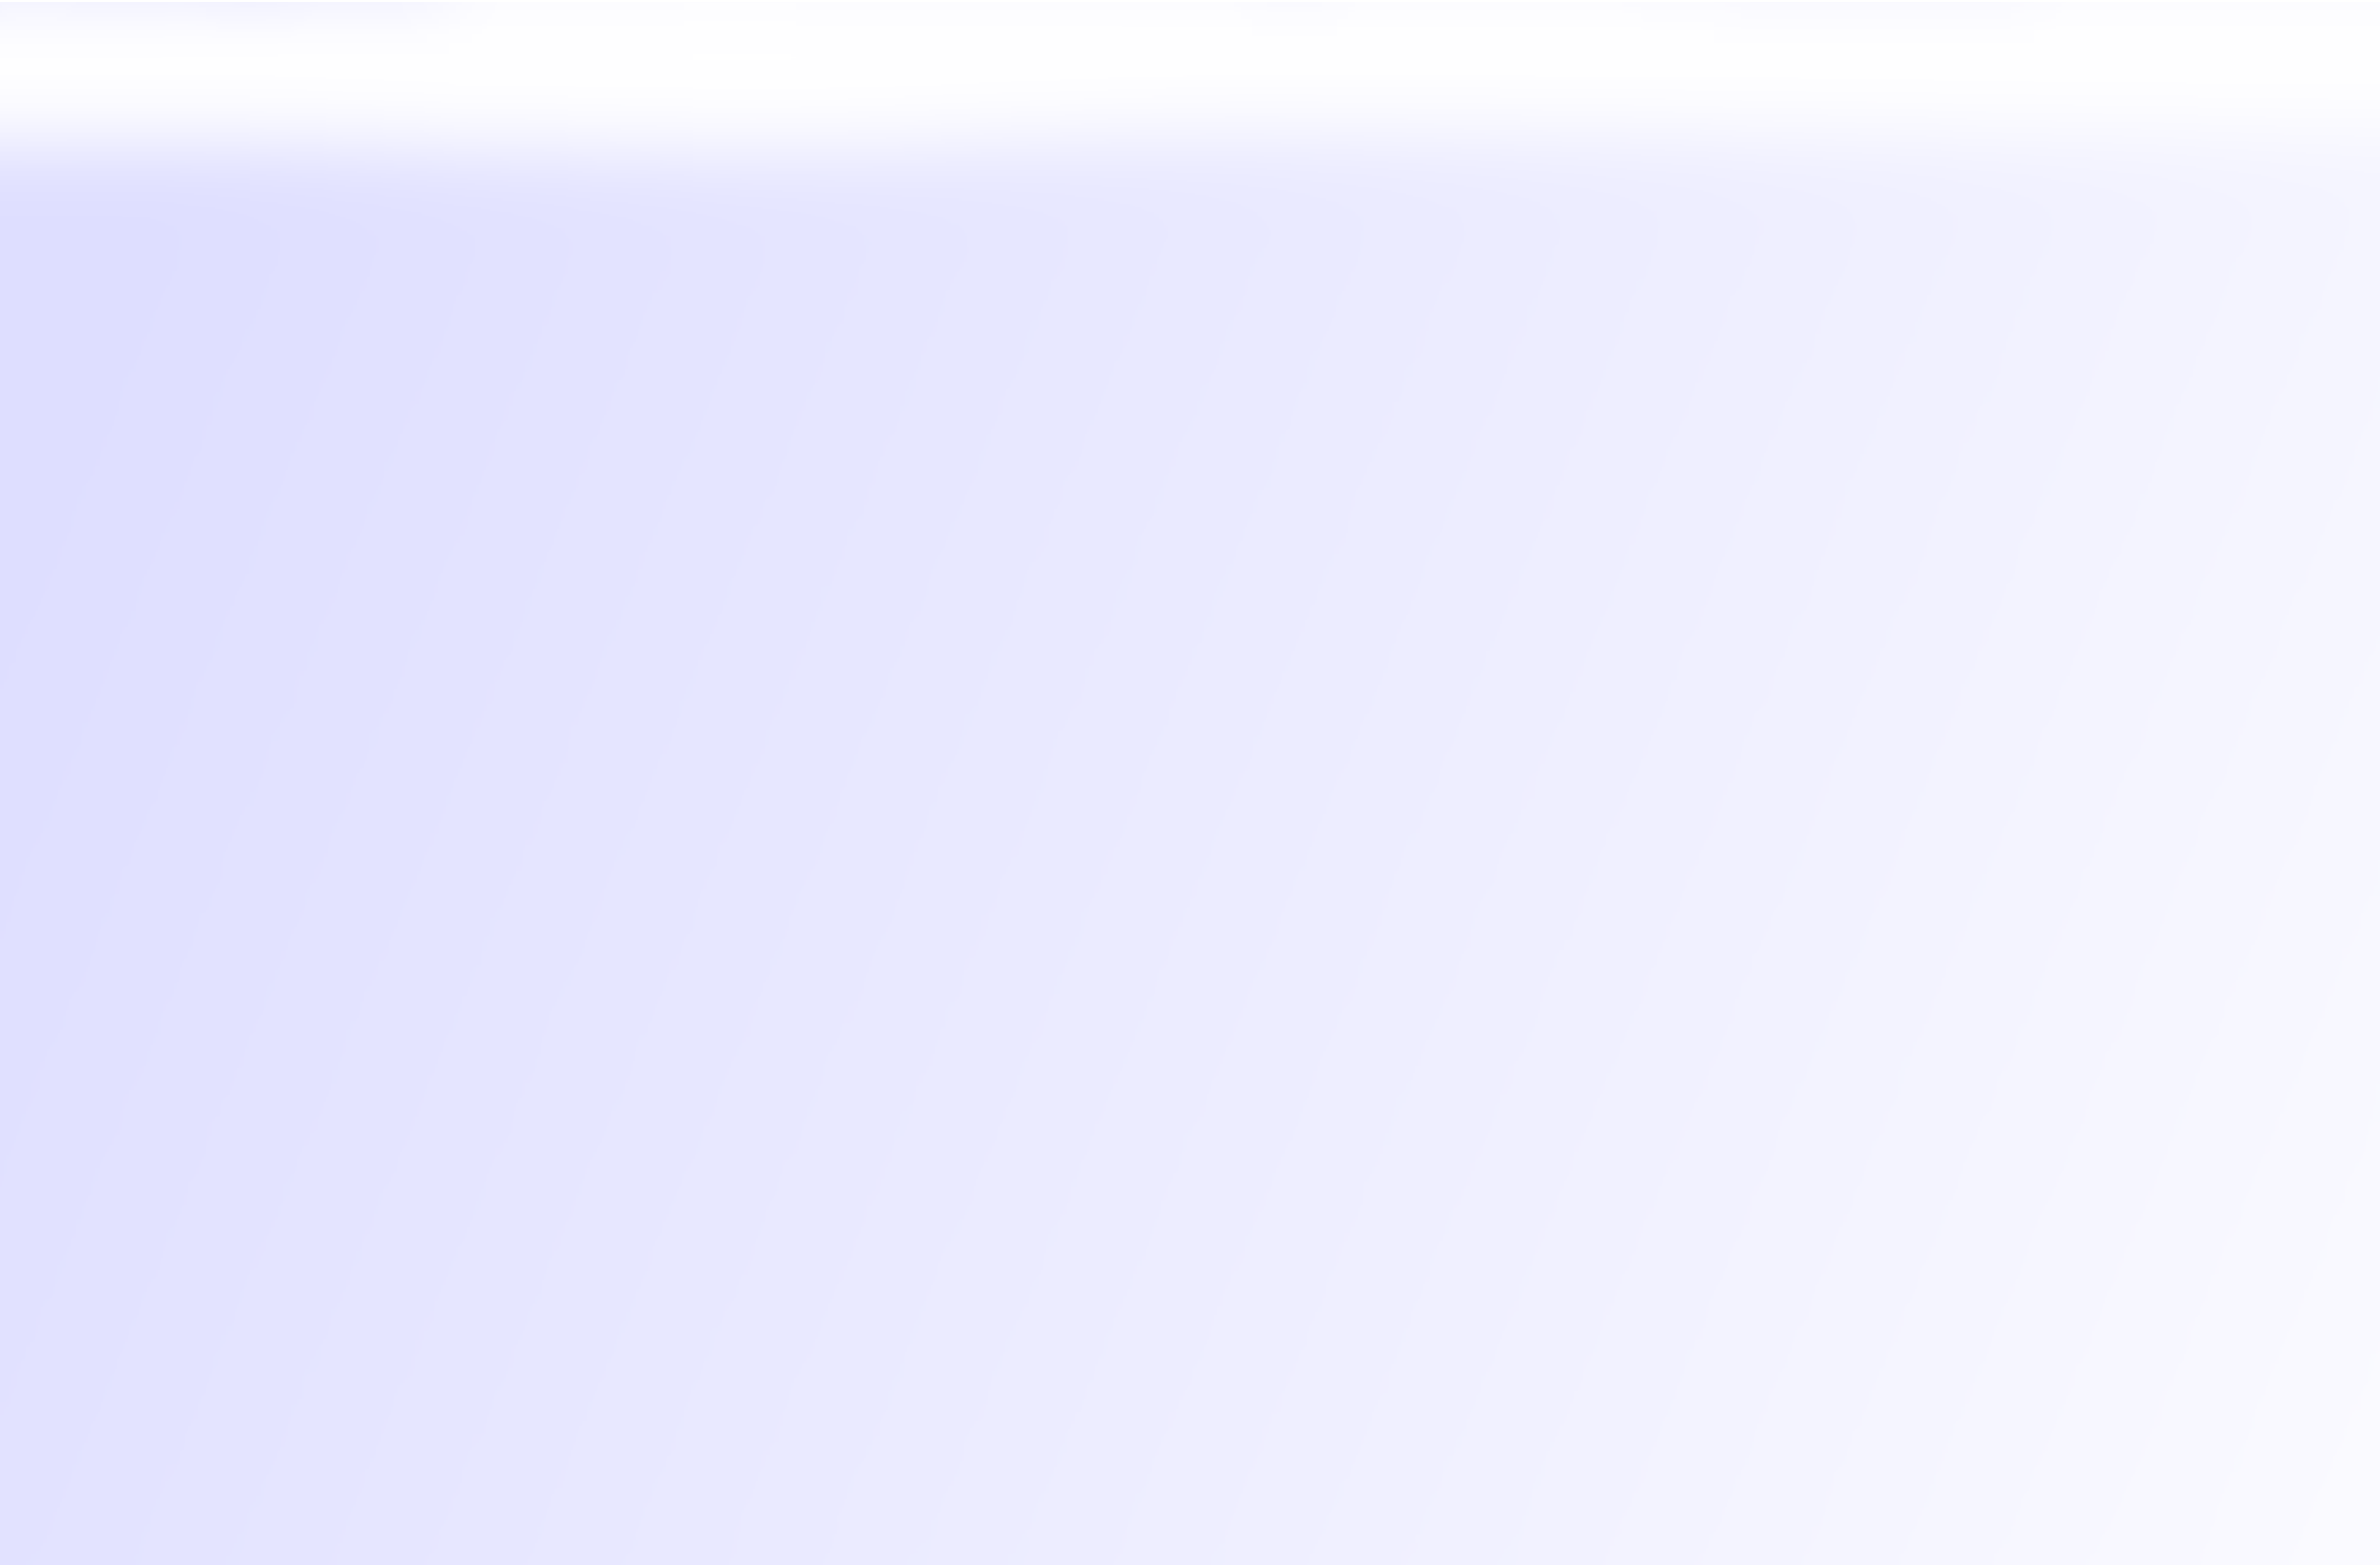
\includegraphics[height=1.1\textheight]{background}};
\end{tikzpicture}
}

\begin{poster}{
grid=false,
borderColor=bordercol, % Border color of content boxes
headerColorOne=headercol1, % Background color for the header in the content boxes (left side)
headerColorTwo=headercol2, % Background color for the header in the content boxes (right side)
headerFontColor=headerfontcol, % Text color for the header text in the content boxes
boxColorOne=boxcolor, % Background color for the content in the content boxes
headershape=roundedright, % Specify the rounded corner in the content box headers
headerfont=\Large\sf\bf, % Font modifiers for the text in the content box headers
textborder=rectangle,
background=user,
headerborder=open, % Change to closed for a line under the content box headers
boxshade=plain
}
{
\includegraphics[scale=0.2]{erato.png}}
%
%----------------------------------------------------------------------------------------
%	TITLE AND AUTHOR NAME
%----------------------------------------------------------------------------------------

{\huge    {closed for a line under the content box headers} } % Poster title
{\vspace{0.3em} \smaller Zhenya Zhang  \\  % Author names
  
\smaller $^1$\it {National Institute of Informatics, Tokyo, Japan}\\\it{The Graduate University for Advanced Studies, Hayama, Japan}  } } 


%----------------------------------------------------------------------------------------
%	INTRODUCTION
%----------------------------------------------------------------------------------------
\headerbox{Overview}{name=introduction,column=0,row=0, span=3}{



%In formal verification one aims to give a mathematical proof for a system's correctness. This is much harder for hybrid systems than for computer software/hardware, %. One reason is theoretical:
% where the presence of continuous dynamics makes many problems more complex or even undecidable (e.g.\ reachability in hybrid automata). 
% \begin{minipage}{0.65\textwidth}
%    \underline{\bfseries The falsification problem}


 % \end{minipage}




}


%----------------------------------------------------------------------------------------
%	CALIBRATION
%----------------------------------------------------------------------------------------
\headerbox{Falsification}{name=relwork, column=0, below=introduction}{
Falsification problem is defined as follows:
    \begin{itemize}
    \item{\textbf{Given:}} 
      a \emph{Simulink} model $\mathcal{M}$ or other black box, and
      a \emph{specification} $\varphi$ in Signal Temporal Logic (STL)

    \item{\textbf{Answer:}} 
      \emph{error input}, i.e., an input signal $\bu$ such
      that the corresponding output $\mathcal{M}(\bu)$ violates $\varphi$ 
    \end{itemize}
\begin{minipage}{0.4\textwidth}
\centering
  \begin{math} 
 \hspace{2em} \xymatrix@1@+2.5em{
   {}
     \ar[r]^-{\bu}
   &
   {  \quad\xybox{ *++++[F]{\mathcal{M}} }}
     \ar[r]^-{\mathcal{M}(\bu)}_-{\not\models\varphi \; ?}
   &
   {}
   }
  \end{math}
 \end{minipage}


}


\headerbox{``Barbaric Reachability''}{name=meric, column=0, below=relwork}{

  
}



\headerbox{Signal Temporal Logic (STL)}{name=optsolver, column=0, below=meric}{
STL is used for formalizing system requirements, like safety or comfort concerns 

E.g., $\varphi \equiv \Box_{[0, 30]}(\speed[t] < 120)$

\begin{tabular}{c|c|c}
%\hline
 signal $\bw$  &$\bw\models\varphi$
 & $\sem{\bw,\varphi}$
\\ \hline
 %Boolean\\satisfaction
 \begin{minipage}{0.4\textwidth}\vspace{+0.2em}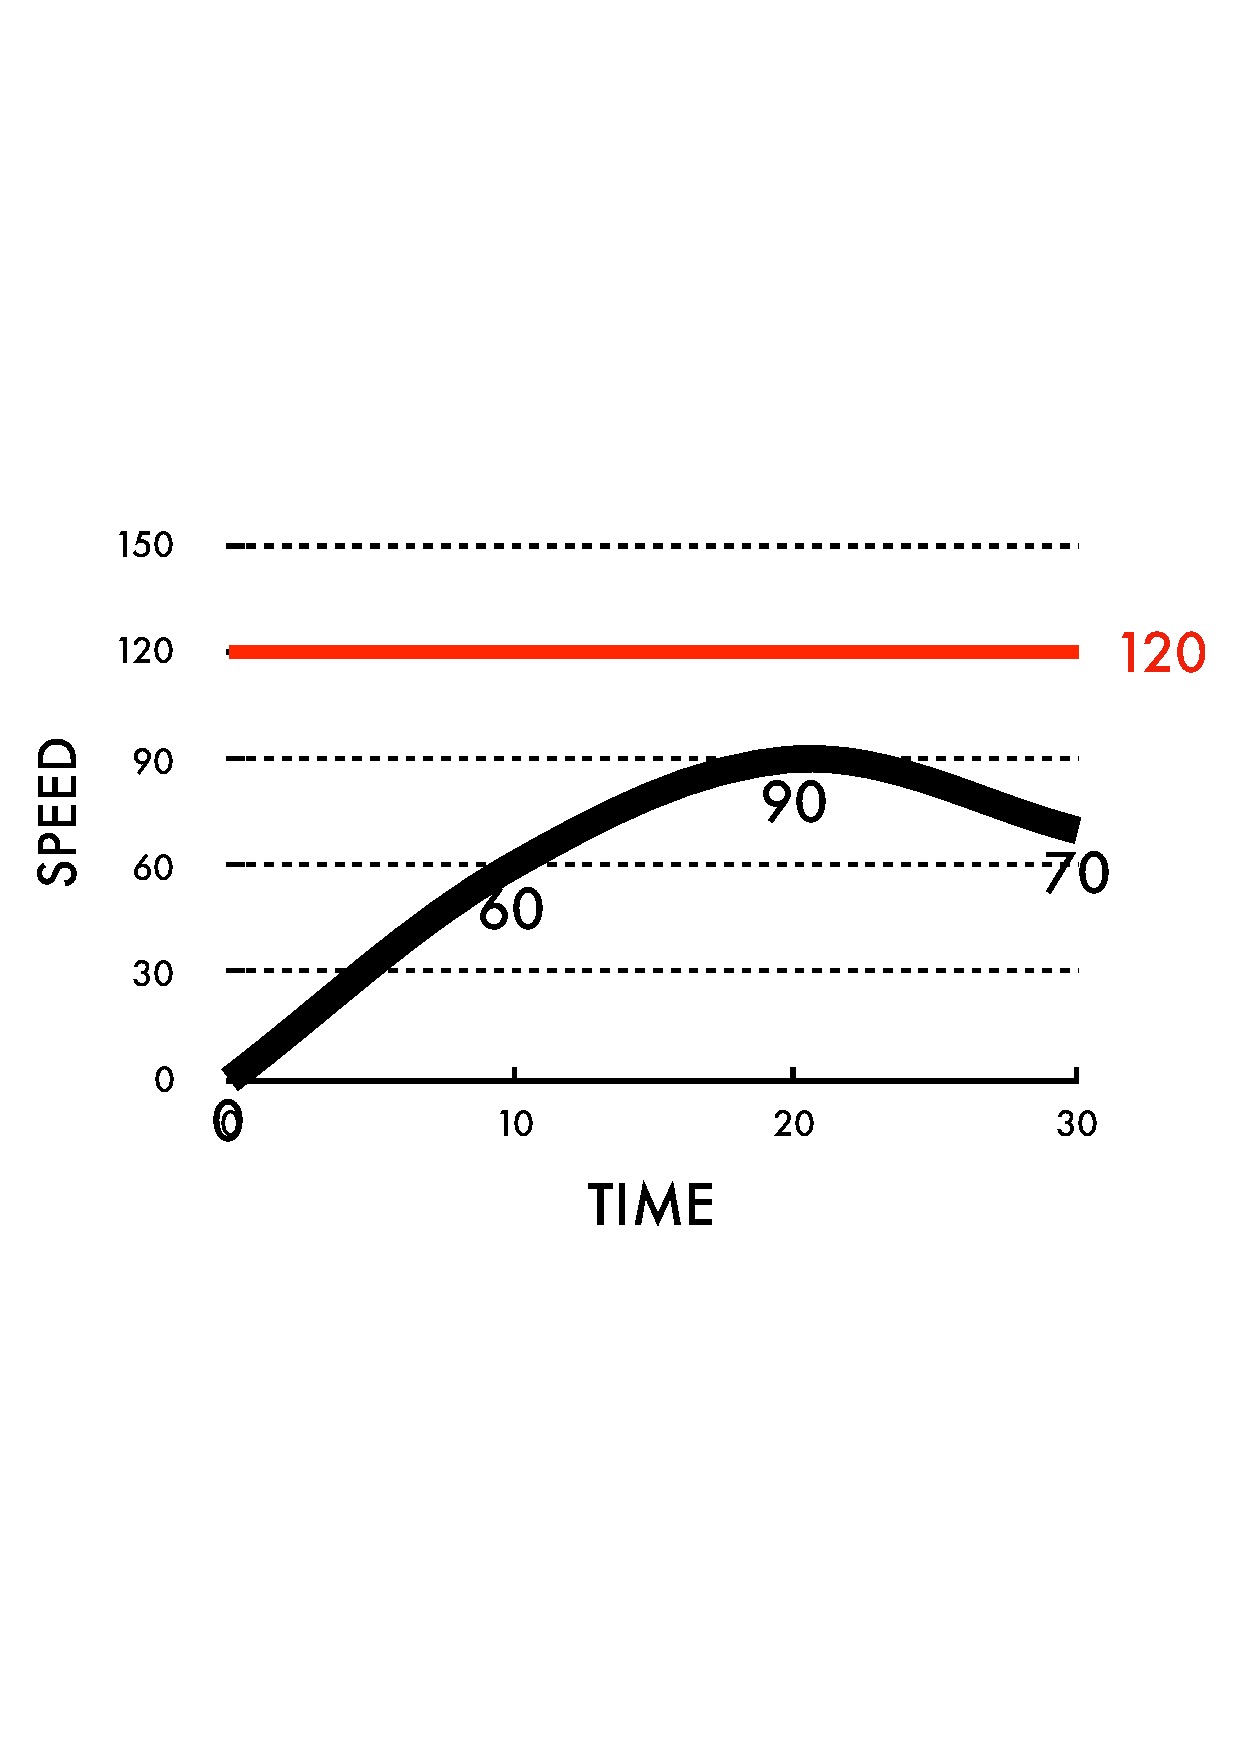
\includegraphics[width=0.99\textwidth]{figures/stleg1.pdf} \end{minipage}\vspace{+0.2em}
& TRUE & 30  \\ \hline
%quantitative\\robustness
 \begin{minipage}{0.4\textwidth}\vspace{+0.2em}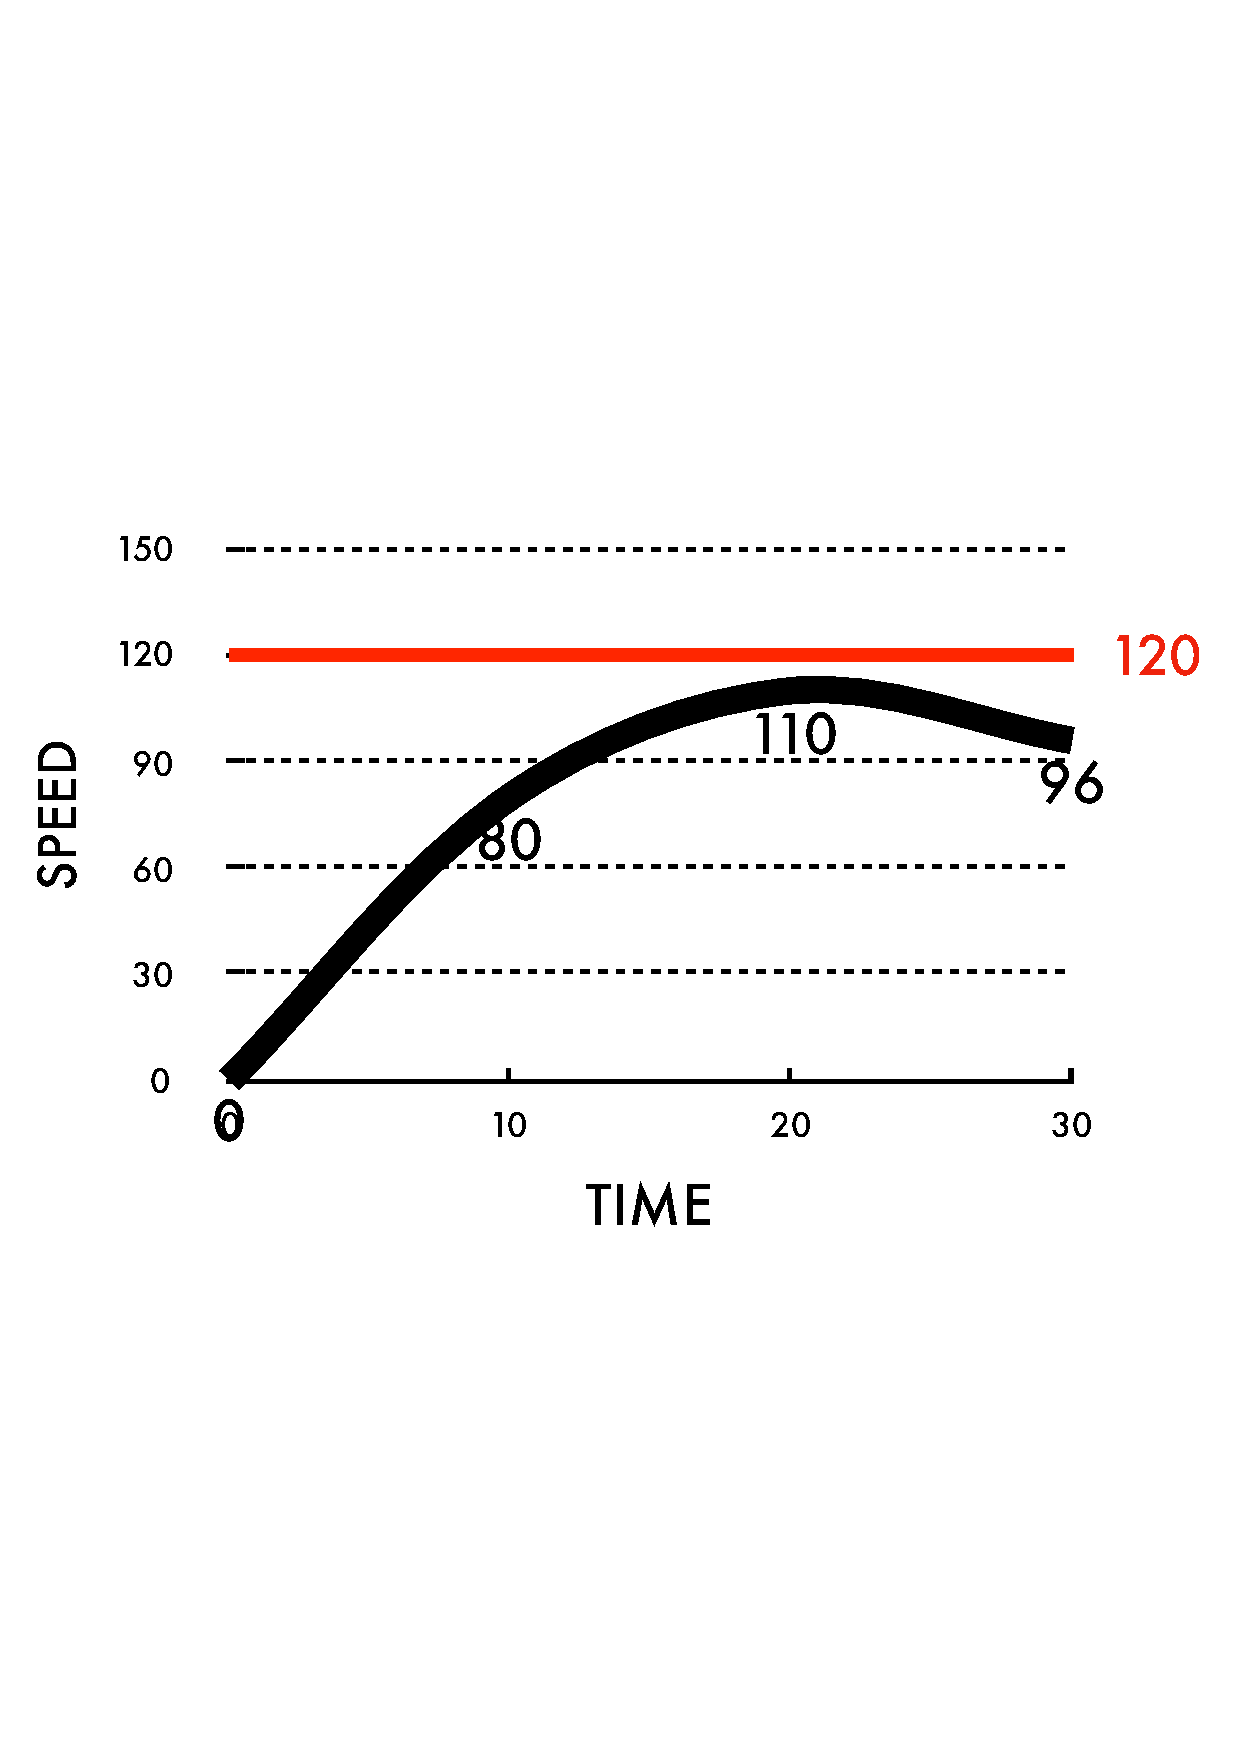
\includegraphics[width=0.99\textwidth]{figures/stleg2.pdf} \end{minipage}  \vspace{+0.2em}
& TRUE & 10 \\ \hline
\begin{minipage}{0.4\textwidth}\vspace{+0.2em}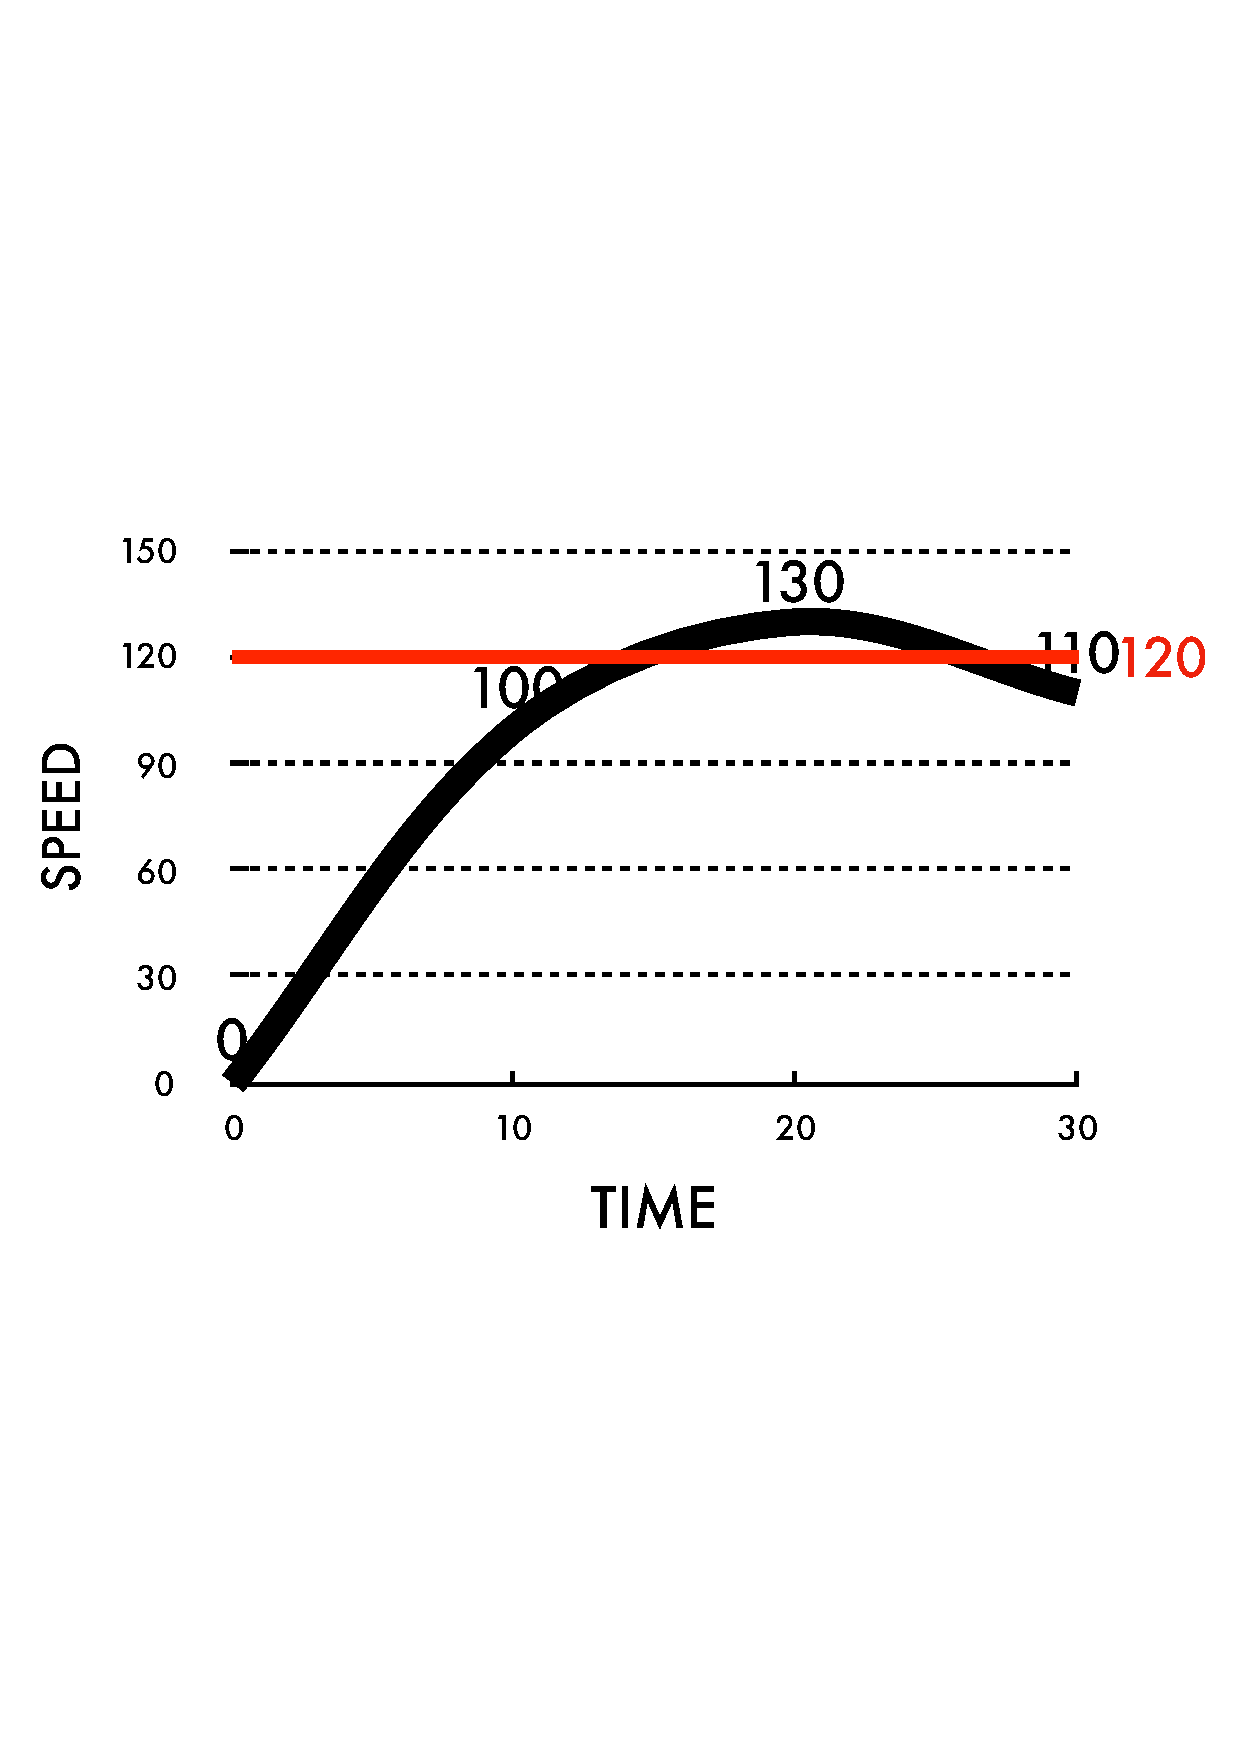
\includegraphics[width=0.99\textwidth]{figures/stleg3.pdf} \end{minipage}\vspace{+0.2em}  
& FALSE & -10 

%\\ \hline
\end{tabular}

  
}

\headerbox{``Hill-climbing'' Optimization}{name=overview, column=0, below=optsolver}{
Falsification $\Rightarrow$ optimization problem:



}


%----------------------------------------------------------------------------------------
%	OTHER INSTRUMENTATION
%----------------------------------------------------------------------------------------
\headerbox{Instance 1}{name=algorithm,span=2,column=1,row=1, below=introduction}{ % To reduce this block to 1 column width, remove 'span=2'

\begin{minipage}[h]{0.22\textwidth}
\centering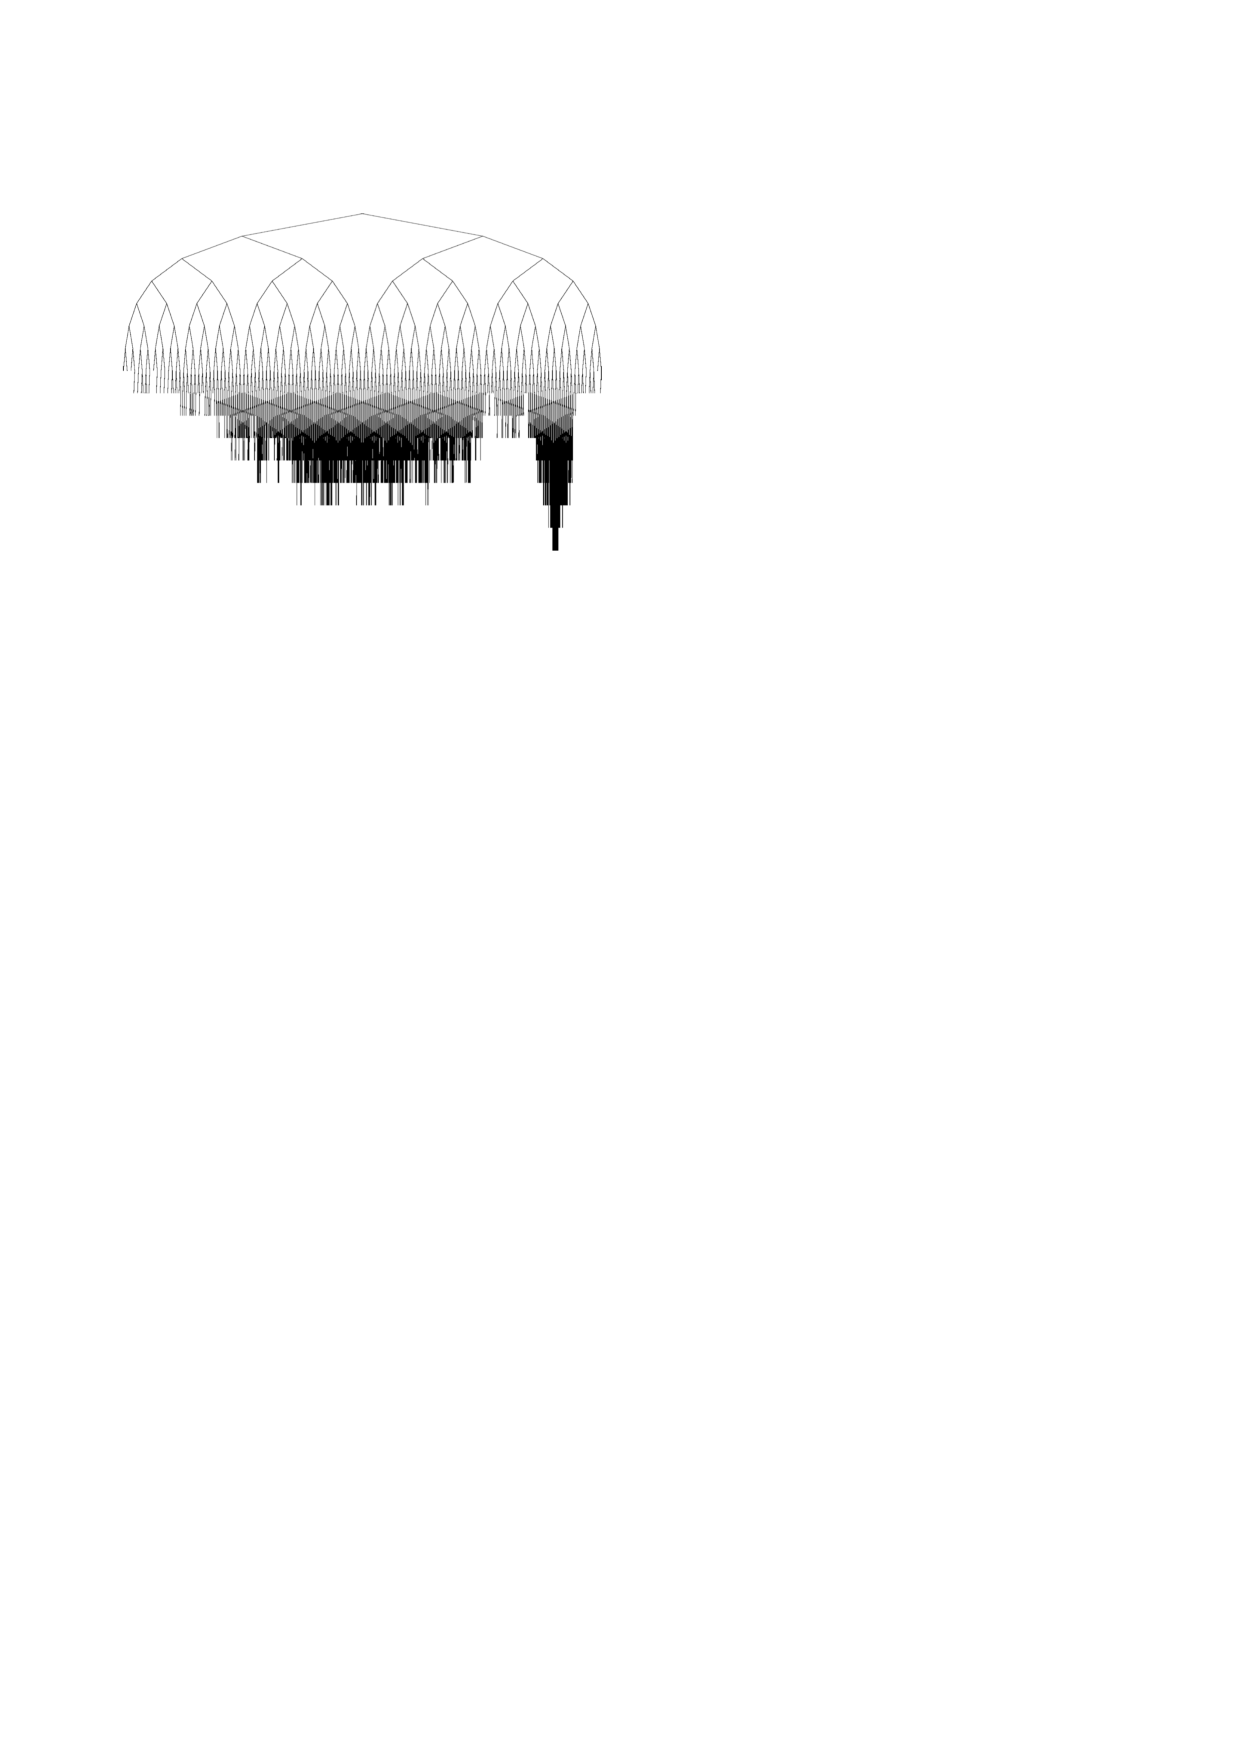
\includegraphics[scale=0.4]{figures/mcts.pdf}
\end{minipage}
\begin{minipage}[h]{0.78\textwidth}
\centering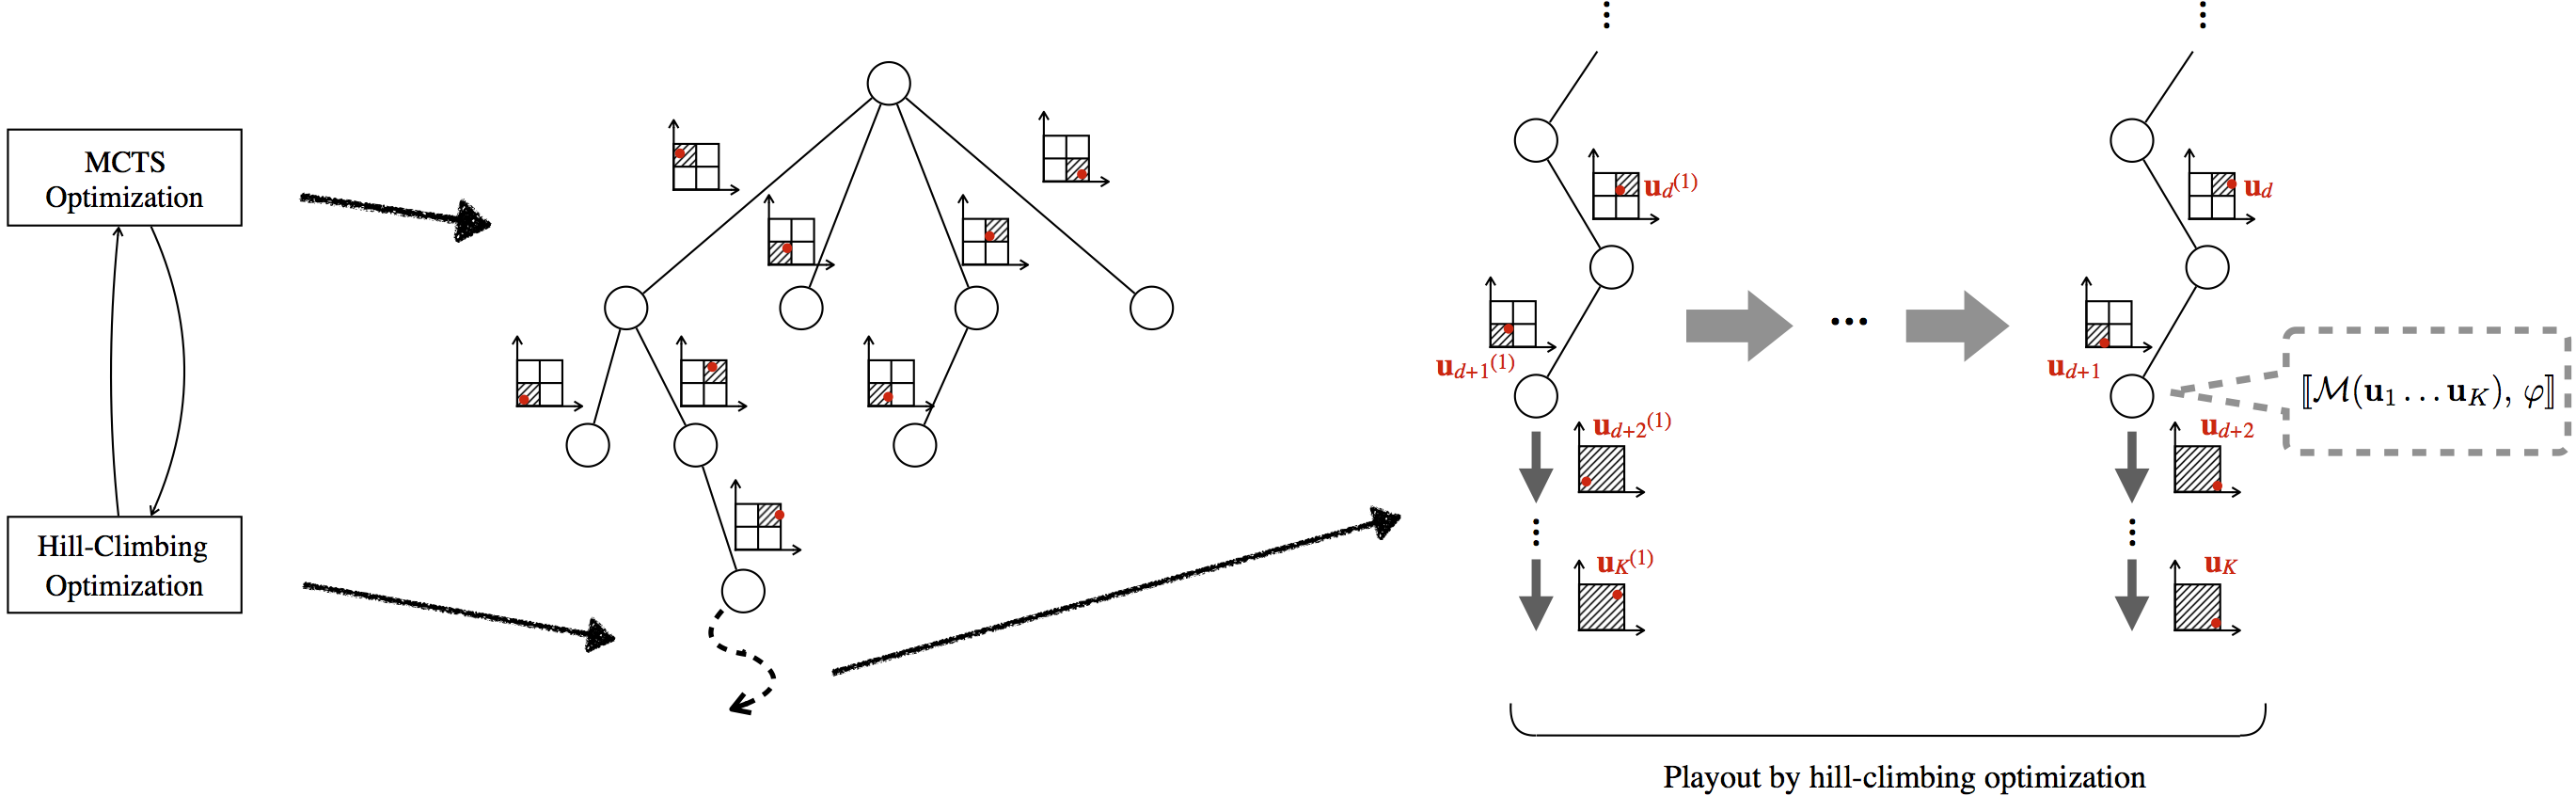
\includegraphics[scale=.1]{figures/algorithm.png}
\end{minipage}




\begin{itemize}
\vspace{-0.6em}
\item Time-staging. Divide the time bound into $K$ intervals to find a sequence $\bu_{1},\dotsc,\bu_{K}$.


\vspace{-0.6em}
\item Node expansion. Use a \emph{partitioning} of the input space $I_{1}\times\cdots\times I_{M}$ as the children set $A$.
\vspace{-0.6em}

\item Child selection. Define that $reward = 1-\frac{R(wa)}{\max_{w'\in\mathcal{T}}R(w')}$, and apply UCB1 algorithm $\argmax_{a\in A} \left(reward + c\sqrt{\frac{2\ln N(w)}{N(wa)}}\right)$ to select the best child.
\vspace{-0.6em}

\item Simulation. Apply optimization solvers in the selected sub-region sequence with time budget.

\vspace{-0.6em}


\item Backpropagation. Update the reward of parent if the newly computed reward is better.

\vspace{-0.6em}

\item Postprocessing. Apply optimization algorithm again if no solution is returned.

\end{itemize}

}


%----------------------------------------------------------------------------------------
%	MIXER vs. SAMPLERS
%----------------------------------------------------------------------------------------
\headerbox{Instance 2}{name=autotrans, span=2, column=1, row=1, below=algorithm}{








%\end{small}
}


%----------------------------------------------------------------------------------------
%	MEASUREMENT SETUP
%----------------------------------------------------------------------------------------



%----------------------------------------------------------------------------------------
%	CONCLUSION
%----------------------------------------------------------------------------------------
\headerbox{Case Study}{name=conclusion,column=1,below=autotrans,span=2}{
\begin{minipage}[h]{0.53\textwidth}

\end{minipage}
\begin{minipage}[h]{0.45\textwidth}

\end{minipage}

}

\headerbox{References}{name=casestudy,column=1,below=conclusion,span=2}{
Related papers:
\begin{footnotesize}
\begin{itemize}


\item Zhang, Z., Ernst, G., Sedwards, S., Arcaini, P., \& Hasuo, I. (2018). Two-layered falsification of hybrid systems guided by monte carlo tree search. IEEE Trans. on CAD of Integrated Circuits and Systems.


\item Zhang, Z., Hasuo, I., Arcaini, P. (2019). Multi-Armed Bandits for Boolean Connectives in Hybrid System Falsification. 31st International Conference on Computer-Aided Verification (CAV) 2019.

\end{itemize}

%Others:
%\begin{itemize}
%\item Ernst, G., Hasuo, I., Zhang, Z., \& Sedwards, S. (2018). Time-staging enhancement of hybrid system falsification. 

%\item Ernst, G., Sedwards, S., Zhang, Z., \& Hasuo, I. (2018). Fast Falsification of Hybrid Systems using Probabilistically Adaptive Input. 

%\item Dokhanchi, A., Yaghoubi, S., Hoxha, B., Fainekos, G., Ernst, G., Zhang, Z., Arcaini, P., Hasuo, I. \& Sedwards, S. (2018). ARCH-COMP18 Category Report: Results on the Falsification Benchmarks. 

%\item Ernst, G., Arcaini P., Donze, A., Fainekos, G., Mathesen, L., Pedrielli, G., Yaghoubi, S., Yamagata, Y., \&  Zhang, Z.. (2019). ARCH-COMP19 Category Report: Falsification. 
%\end{itemize}
\end{footnotesize}
}


%----------------------------------------------------------------------------------------
%	REFERENCES
%----------------------------------------------------------------------------------------

%\headerbox{References}{name=references,column=2,below=application}{

%\smaller % Reduce the font size in this block
%\renewcommand{\section}[2]{\vskip 0.05em} % Get rid of the default "References" section title
%\nocite{*} % Insert publications even if they are not cited in the poster

%\bibliographystyle{unsrt}
%\bibliographystyle{IEEEtran}
%\bibliography{biblio} % Use biblio.bib as the bibliography file
%}


%----------------------------------------------------------------------------------------
%	ACKNOWLEDGEMENTS
%----------------------------------------------------------------------------------------

\headerbox{Acknowledgements}{name=acknowledgements,column=0,below=casestudy, above=bottom,span=3}{

This work is supported by ERATO HASUO Metamathematics for Systems Design Project
(No. JPMJER1603), Japan Science and Technology Agency.
} 


\end{poster}

\end{document}